
\section{Application Study}
\label{sec:application study}

\begin{comment}
A parallel application usually conforms to a combination of several basic communication patterns~\cite{roth}. 
At its different execution phases, 
the application's communication behavior may follow certain basic pattern respectively. 
There are many profiling tools available to capture 
information regarding communication patterns of parallel applications~\cite{tau,mpip,sst,oxbow}. 
They can provide information such as the percentage of different MPI operations, 
communication topology, the amount of data transferred between processes, etc.

There are many applications running on HPC systems such as Mira~\cite{bgq} and Titan~\cite{titan}. 
These applications are communication intensive and conform to various communication patterns. 
\end{comment}

In this work, we select three applications from the DOE Design Forward Project. 
Each application exhibits a distinctive communication pattern that is commonly seen in HPC applications. 
We believe that the communication patterns of these applications 
are representative of a wide array of applications running on leadership-class machines. 
Specifically, we study the Algebraic MultiGrid Solver (AMG), 
Geometric MultiGrid (MultiGrid) and CrystalRouter MiniApps. 
The communication matrixes of each application presented in Figure~\ref{fig:amg-communication-topology}
,\ref{fig:cr-communication-topology} and \ref{fig:mg-communication-topology} are generated by
the IPM data collected from~\cite{designforwardwebpage}.
%are generated with the IPM~\cite{ipm} data gathered from publicly available traces~\cite{designforwardwebpage}.


%\begin{figure*}[htp]
%    \centering
%    \begin{subfigure}[t]{0.32\textwidth}
%        \centering
%        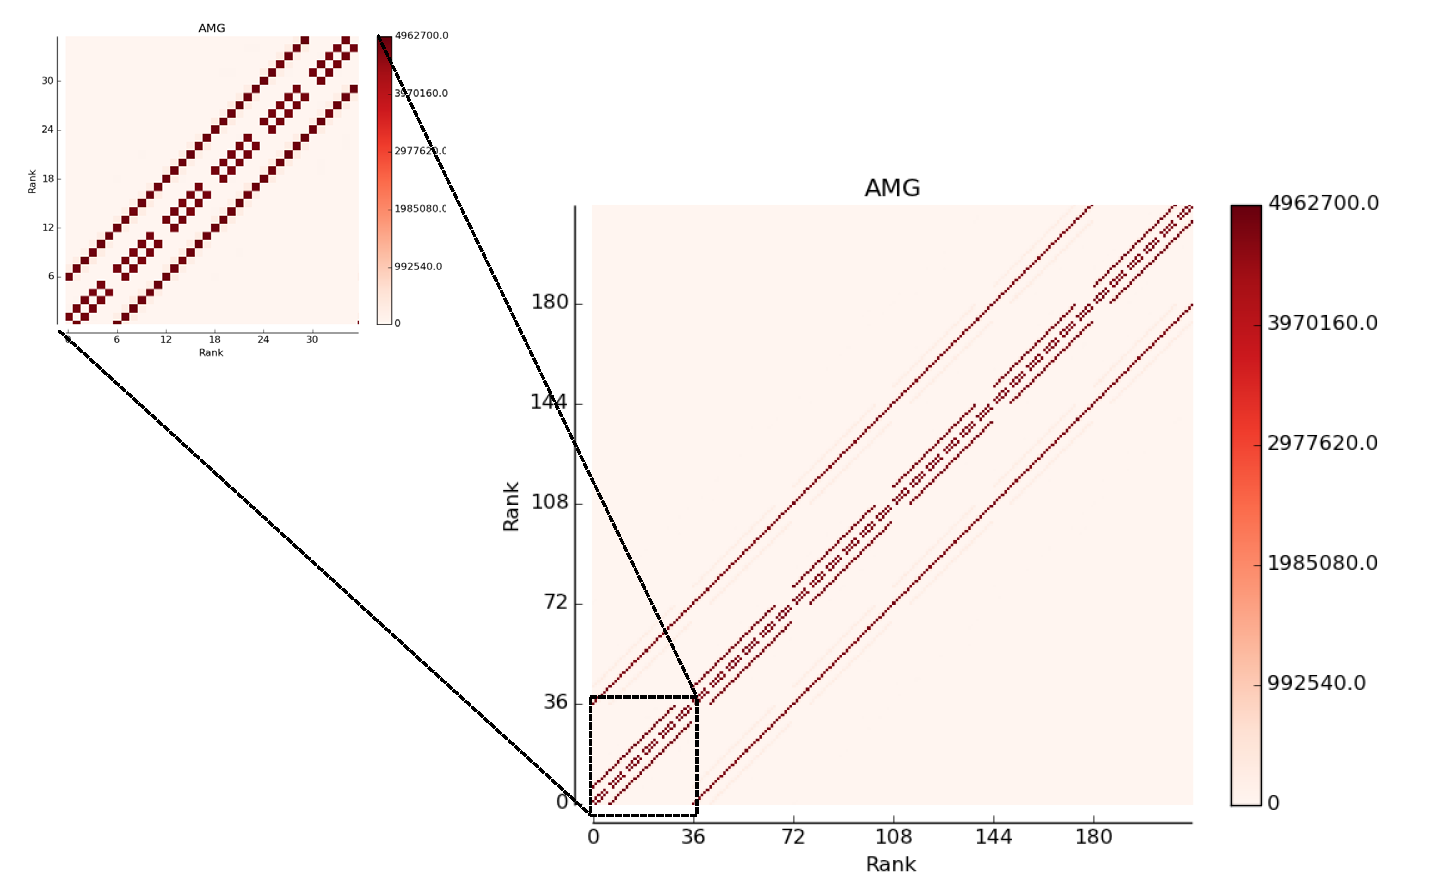
\includegraphics[height=1.5in]{figs/appstudy/amg/amg_pip}
%        \caption{AMG}
%        \label{fig:amg-communication-topology}
%    \end{subfigure}
%    \begin{subfigure}[t]{0.32\textwidth}
%        \centering
%        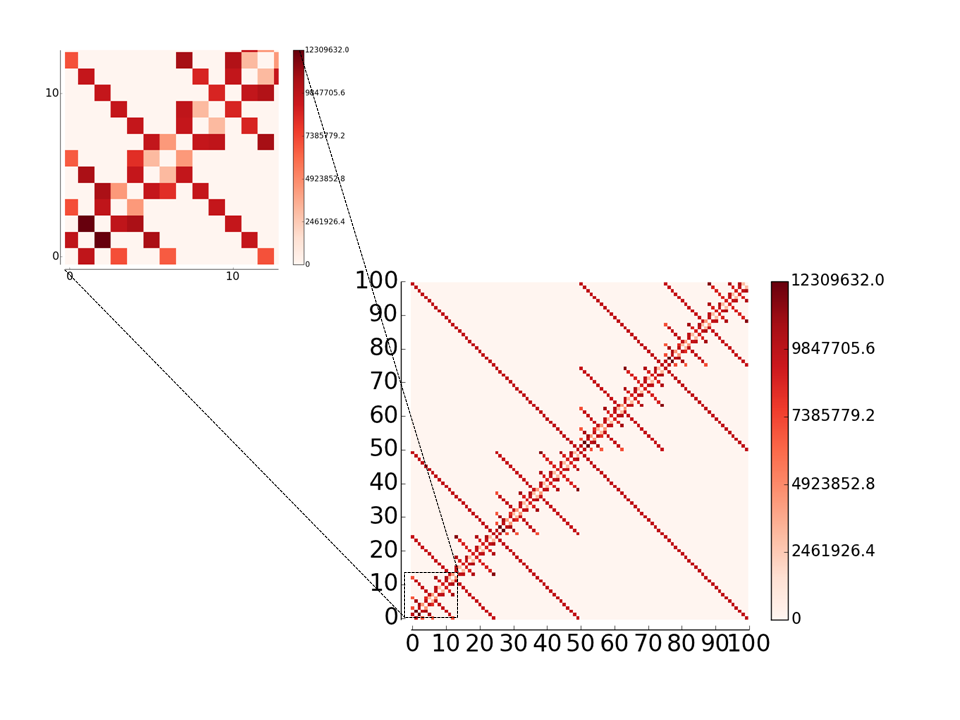
\includegraphics[height=1.5in]{figs/appstudy/cr/cr_pip}
%        \caption{CrystalRouter}
%        \label{fig:cr-communication-topology}
%    \end{subfigure}
%    \begin{subfigure}[t]{0.32\textwidth}
%        \centering
%        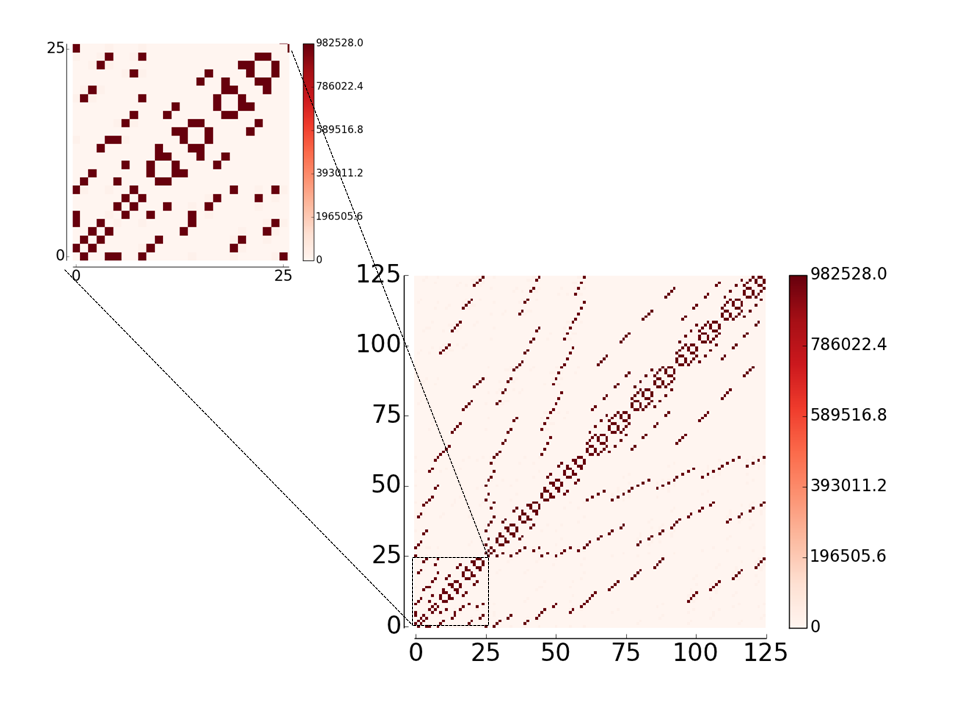
\includegraphics[height=1.5in]{figs/appstudy/mg/mg_pip}
%        \caption{MultiGrid}
%        \label{fig:mg-communication-topology}
%    \end{subfigure}
%    \caption{Applications rank-to-rank communication topology graph.}
%    \label{fig:apps_communication_matrix}
%\end{figure*}


\subsection{AMG}
\label{sec:amg}

\begin{figure}[htp]
    \centering
    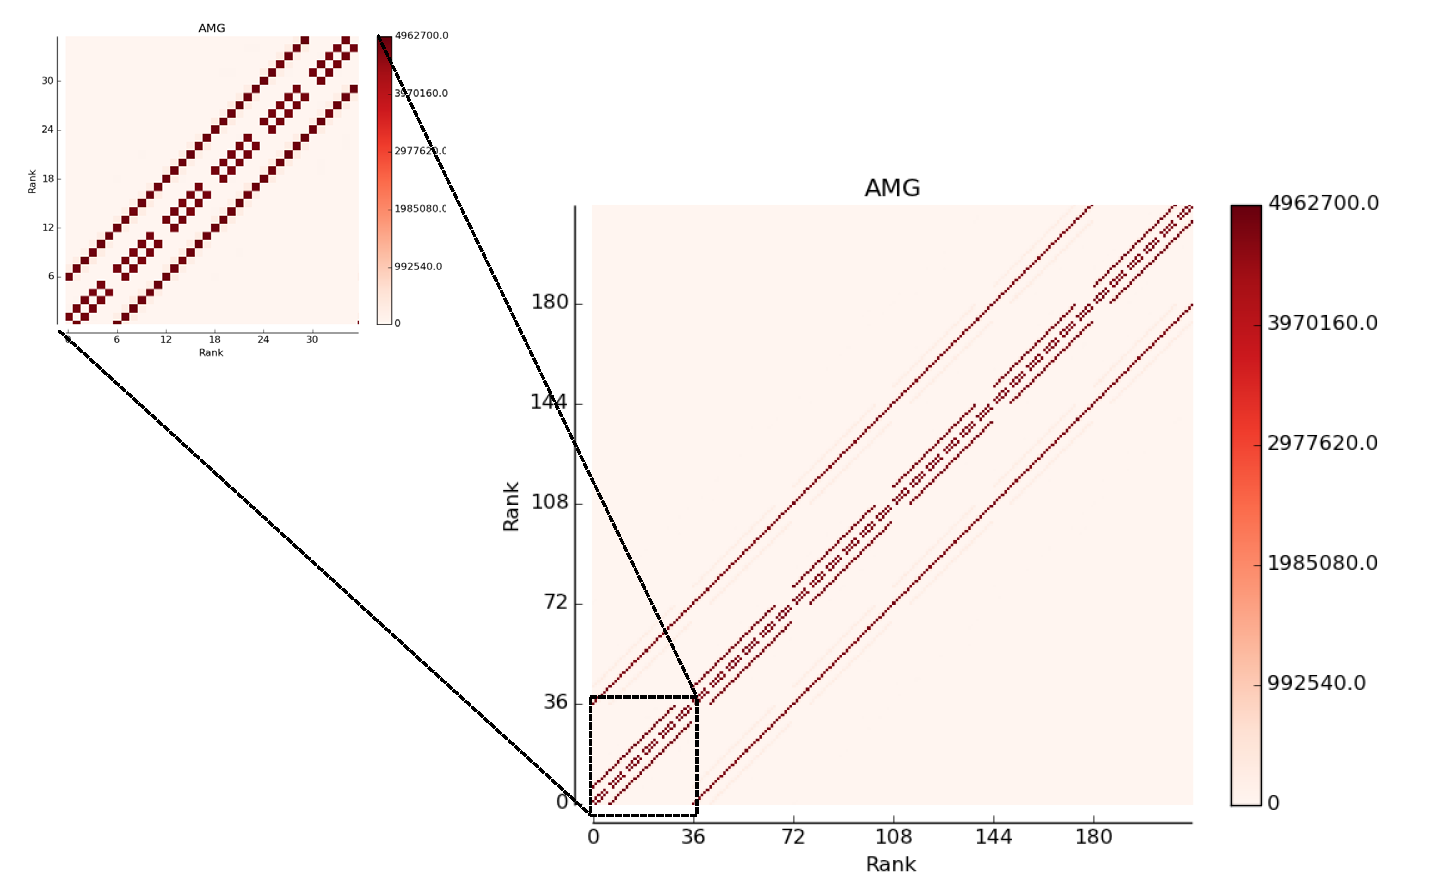
\includegraphics[height=2.5in]{figs/appstudy/amg/amg_pip}
    \caption{AMG Communication Matrix. 
        The label of both x and y axis is the index of MPI rank in AMG. 
        The legend bar on the right indicates the data transfer 
        amount between ranks.
        }
    \label{fig:amg-communication-topology}
\end{figure}

The Algebraic MultiGrid Solver, or AMG, 
is a parallel algebraic multi-grid solver for linear systems arising 
from problems on unstructured mesh physics packages. 
It has been derived directly from the BoomerAMG solver 
that is being developed in the Center for Applied Scientific Computing (CASC) at LLNL \cite{amg}. 
The dominant communication pattern is regional communication 
with decreasing message size for different parts of the multi-grid v-cycle.

Figure~\ref{fig:amg-communication-topology} shows the communication matrix 
of a small scale AMG execution with 216 MPI ranks. 
Note that the dominant communication pattern of the application doesn't change with scale. 
We observe that AMG's dominant communication pattern is 3D nearest neighbor - 
each rank has intensive communication with up to six neighbors, depending on rank boundaries. 
Applications with similar patterns include PARTISN~\cite{partisn} and SNAP~\cite{snap}.


\subsection{Crystal Router}
\label{sec:crystalrouter}

\begin{figure}[htp]
    \centering
    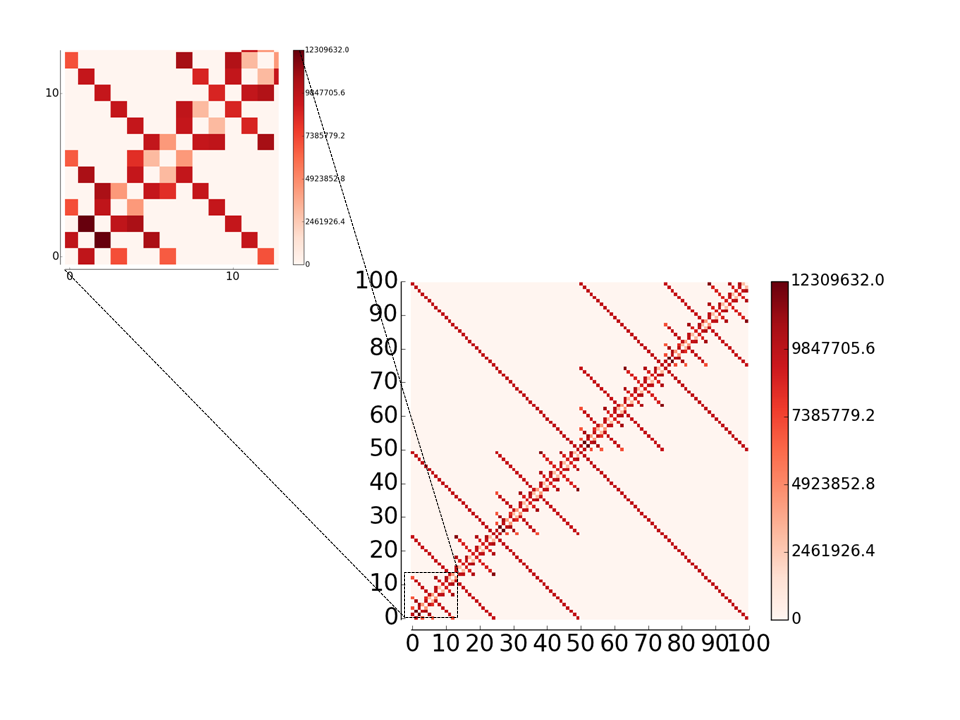
\includegraphics[height=2.5in]{figs/appstudy/cr/cr_pip}
    \caption{CrystalRouter Communication Matrix. 
        The label of both x and y axis is the index of MPI rank in CrystalRouter. 
        The legend bar on the right indicates the data transfer 
        amount between ranks.
        }
    \label{fig:cr-communication-topology}
\end{figure}

The second MiniApp covered is CrystalRouter, 
the extracted communication kernel of the full application Nek5000~\cite{nek5000}, 
which is a spectral element CFD application developed at Argonne National Laboratory. 
It features spectral element multi-grid solvers coupled with a highly scalable, 
parallel coarse-grid solver that is widely used for projects including ocean current modeling, 
thermal hydraulics of reactor cores, and spatiotemporal chaos. 
CrystalRouter demonstrates the many-to-many communication pattern 
through a scalable multi-stage communication process. 

The collective communication in CrystalRouter utilizes a recursive doubling approach. 
Ranks in CrystalRouter conform to a $n$-dimensional hypercube 
and recursively split into ($n$-1)-dimensional hypercubes, 
with communication occurring along the splitting plane. 
The pattern of this communication can be found in Figure~\ref{fig:cr-communication-topology}. 
By nature of the logarithmic splitting process, 
a substantial portion of the communication occurs in small neighborhoods of ranks. 
CrystalRouter represents a group of applications whose dominant communication 
is a hybrid of multi-stage local and hierarchical global communication, 
and shares similarities with most MPI collective communication implementations.


\subsection{MultiGrid}
\label{sec:multigrid}

\begin{figure}[htp]
    \centering
    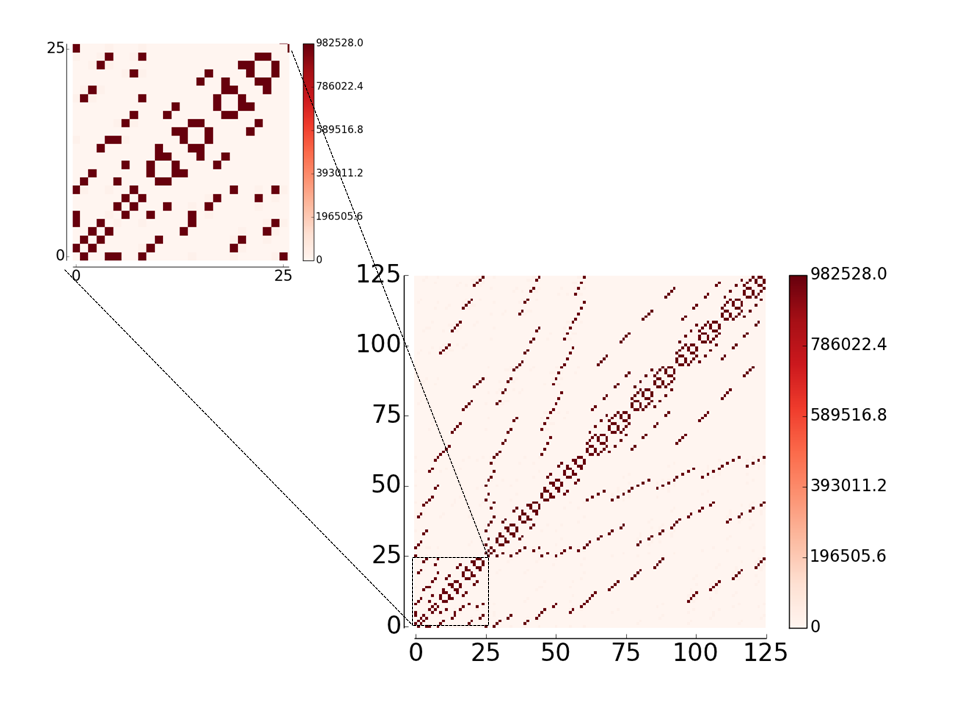
\includegraphics[height=2.5in]{figs/appstudy/mg/mg_pip}
    \caption{MultiGrid Communication Matrix. 
    The label of both x and y axis is the index of MPI rank in MultiGrid. 
    The legend bar on the right indicates the data transfer amount between ranks.
    }
    \label{fig:mg-communication-topology}
\end{figure}

MultiGrid is geometric multi-grid v-cycle from the production elliptic solver BoxLib, 
a software framework for massively parallel block-structured adaptive mesh refinement (AMR) codes~\cite{boxlib}. 
MultiGrid conforms to many-to-many communication pattern with decreasing message size and 
collectives for different parts of the multi-grid v-cycle. 
It is widely used for structured grid physics packages. 

Figure~\ref{fig:mg-communication-topology} shows the communication matrix of MultiGrid with 125 ranks. 
We can see intensive communication along the diagonal that resembles nearest neighbor communication, similar to AMG. 
However, the communication topology leads to a greater ``spread'' of communication across the set of ranks, 
challenging the maximization of communication locality with respect to ranks. 
In this sense, it can be considered as many-to-many pattern. 
Applications with such similar dominant communication patterns are like FillBoundary, another PDE solver code in~\cite{boxlib}.


